\documentclass[stu, a4paper, 12pt, floatsintext]{apa7}

% Title Page Stuff
\title{Flight Systems E3 Assignment Report (Digital Servo and MATLAB Assignment)}
\shorttitle{Flight Systems Coursework}
\leftheader{25/03/25}
\authorsnames{Philip Beswick @00662943}
\authorsaffiliations{The University of Salford}
\course{Flight Systems E3}
\professor{Professor T X Mei, Dr B A Sangolola, Dr Y Govdeli, Dr O K Ariff}
\duedate{18/03/25}
\abstract{Some abstract yada yada yada}

% Packages Required
\usepackage{csquotes}
\usepackage[english]{babel}
\usepackage[T1]{fontenc}
\usepackage{mathptmx}
\usepackage{multirow}
\usepackage{graphicx}
\usepackage{booktabs}
\usepackage[style=apa,sortcites=true,sorting=nyt,backend=biber]{biblatex}
\usepackage{pgf-pie}
\usepackage{pgfplots}
\usepackage{paracol}
\usepackage{amsmath}
\usepackage{tocloft}
\usepackage{float}
\usepackage{listings}

\addbibresource{bibliography.bib}

\pgfplotsset{compat=1.18}

% Counts chapters numerically
\setcounter{tocdepth}{5}
\setcounter{secnumdepth}{5}

% Counts equations, figures and tables sequentially depending on the chapter
\numberwithin{figure}{section}
\numberwithin{table}{section}
\numberwithin{equation}{section}

\newcommand{\listequationsname}{\Large List of Equations}
\newlistof{myequations}{equ}{\listequationsname}
\newcommand{\myequations}[1]{%
\addcontentsline{equ}{myequations}{\protect\numberline{\theequation}#1}\par}
\setlength{\cftmyequationsnumwidth}{2.5em}% Width of equation number in List of Equations

% Makes sure LaTeX knows where we are :D
\DeclareLanguageMapping{british}{british-apa}

% Define MATLAB syntax highlighting
\lstdefinelanguage{Matlab}{
  morekeywords={break,case,catch,continue,else,elseif,end,for,function,
    global,if,otherwise,persistent,return,switch,try,while, on, off},
  morekeywords=[2]{abs,acos,asin,atan,ceil,cos,exp,floor,log,log10,max,min,
    mod,round,sign,sin,sqrt,tan, evalfr, angle, feedback, plot, rlocus, cell2mat, figure, hold, title, fprintf, disp, info, step, grid, sprintf, pole, zero},
  keywordstyle=\color{blue}\bfseries,
  keywordstyle=[2]\color{teal},
  identifierstyle=\color{black},
  stringstyle=\color{red},
  commentstyle=\color{green!60!black},
  numbers=left,
  numberstyle=\tiny\color{gray},
  stepnumber=1,
  numbersep=5pt,
  basicstyle=\ttfamily\footnotesize,
  breaklines=true,
  showstringspaces=false
}

\begin{document}

\maketitle{} % Generates the title page

\tableofcontents
\vspace*{0.1cm}
\noindent \hyperlink{page.54}{\textbf{References}} \hfill \textbf{NUMBER} % REMEMBER TO UPDATE THIS!!

%%% Contents of report go here %%%
\newpage
\section{Digital Control Design Laboratory}
Introduction
\subsection{Objectives, Theory, Apparatus}
\subsection{Models and Results}
\subsection{Discussion}
\subsection{Conclusions}

\newpage
\section{Altitude Hold Autopilot Design}
Both safety and efficiency have been significantly improved thanks to the introduction of autopilot systems, which have become an essential aspect of modern aviation. Initially, autopilots were introduced to reduce the flight crew’s workload during long-haul flights but over time they have evolved into highly sophisticated systems, which are capable of completing various complex tasks autonomously. One of the different functionalities of autopilots is altitude hold. This feature is of paramount importance for safety and efficiency, as it ensures a steady and controlled flight path is followed, this means that the desired cruising altitude is maintained. Any deviation in the desired cruising altitude could result in serious safety concerns, the aircraft could come into conflict, and cause fuel inefficiencies, thus reducing profit margins for airlines. \newline

The primary function of altitude hold in autopilots is to maintain a specific altitude, autonomously; this allows pilots to focus on other critical aspects of flight, including communicating with air traffic control. This is vitally important for long flights, as small deviations in altitude accumulate over time, resulting in a very significant altitude change (\cite{nasa2017}). This is especially important when flying through turbulence, which can drastically change the aircraft’s altitude in a very short period of time, this turbulence is also very frequently encountered between 30kft and 40kft (the altitude range of most modern airliners) (\cite{nasa2017}). Altitude hold systems will automatically account for these altitude changes, returning the aircraft to equilibrium; the best autopilot systems do this quickly and efficiently (with as few oscillations as possible).

\newpage

\subsection{Objectives and Theory}

\subsubsection{Objectives}
The key objectives of any altitude hold system are: 
\begin{enumerate}
    \item To maintain a fixed altitude, which ensures compliance with Air Traffic Control regulations.
    \item Minimise pilot workload, by providing automatic altitude maintenance during cruise flight.
    \item Enhance flight stability, by reducing oscillations due to atmospheric disturbances and therefore, improving passenger comfort.
    \item Creating smooth transitions when changing altitude, which improves fuel efficiency. 
\end{enumerate}

\subsubsection{Theory}

The altitude hold system is modelled using the two degrees of freedom linear equations of motion, which describe aircraft longitudinal dynamics.

\begin{equation}
    {\dot w} = \overline Z_{w} w+ V_{R}q+\overline  Z_{\eta } \eta  
\end{equation}
\label{eq:2.1}
\myequations{Two DOF Linear Equation of Motion 1}

\begin{equation}
    {\dot q}- \overline M_{ {\dot w} }{\dot w}=\overline  M_{w}w+ \overline M_{q}q+ \overline  M_{\eta } \eta
\end{equation}
\label{eq:2.2}
\myequations{Two DOF Linear Equation of Motion 2}

\begin{equation}
    q={\dot \theta } 
\end{equation}
\label{eq:2.3}
\myequations{Two DOF Linear Equation of Motion 3}

\begin{equation}
    {\dot h}=  V_{R} \theta -w
\end{equation}
\label{eq:2.4}
\myequations{Two DOF Linear Equation of Motion 4}

These equations describe how the aircraft’s vertical velocity (w), pitch rate (q) and altitude (h) change due to control surface deflections ($\eta$). From these equations, transfer functions can be derived…

\begin{equation}
    G^{q}_{\eta}(s)=  {{(\overline M_{\eta}+\overline M_{\dot w}\overline Z_{\eta})s+(\overline M_{w}\overline Z_{\eta}-\overline M_{\eta}\overline Z_{w})}\over{s^2-(V_{R}\overline M_{\dot w}+\overline Z_{w}+\overline M_{q})s+(\overline M_{q}\overline Z_{w}-V_{R}\overline M_{w})}} 
\end{equation}
\label{eq:2.5}
\myequations{Transfer Function: How Elevator Deflection Impacts Pitch Rate}

Equation 2.5 describes how elevator deflection affections pitch rate.

\begin{equation}
    G^{\theta}_{\eta}(s)=  {{1}\over{s}}  \cdot G^{q}_{\eta}
\end{equation}
\label{eq:2.6}
\myequations{Transfer Function: How Elevator Deflection Impacts Pitch Angle}

Equation 2.6 describes how elevator deflection affects pitch angle.

\begin{equation}
    G^{h}_{\theta}(s)=  {{1}\over{s}}  \cdot  {{-\overline Z_{\eta}s^2+(\overline M_{q}+V_{R}\overline M_{\dot w})\overline Z_{\eta}s+V_{R}(\overline M_{w}\overline Z_{\eta}-\overline M_{\eta}\overline Z_{w})}\over{(\overline M_{\eta}+\overline M_{\dot w}\overline Z_{\eta})s+(\overline M_{w}\overline Z_{\eta}-\overline M_{\eta}\overline Z_{w})}} 
\end{equation}
\label{eq:2.7}
\myequations{Transfer Function: How Pitch Angle Impacts Altitude}

Equation 2.7 describes how pitch angle affects altitude. \newline

The autopilot system has been designed using a sequential loop closure approach, with two distinct stages. The first is the design of a pitch attitude hold system, which is made up of the two inner loops seen in figure 2.1. The second is the closure of the feedback loop around the pitch attitude hold system; again as seen in figure 2.1.

\begin{figure}[H]
    \caption{Block diagram of an Altitude Hold System.}
    \label{fig:block_diagram_altitude_hold}
    \centering
    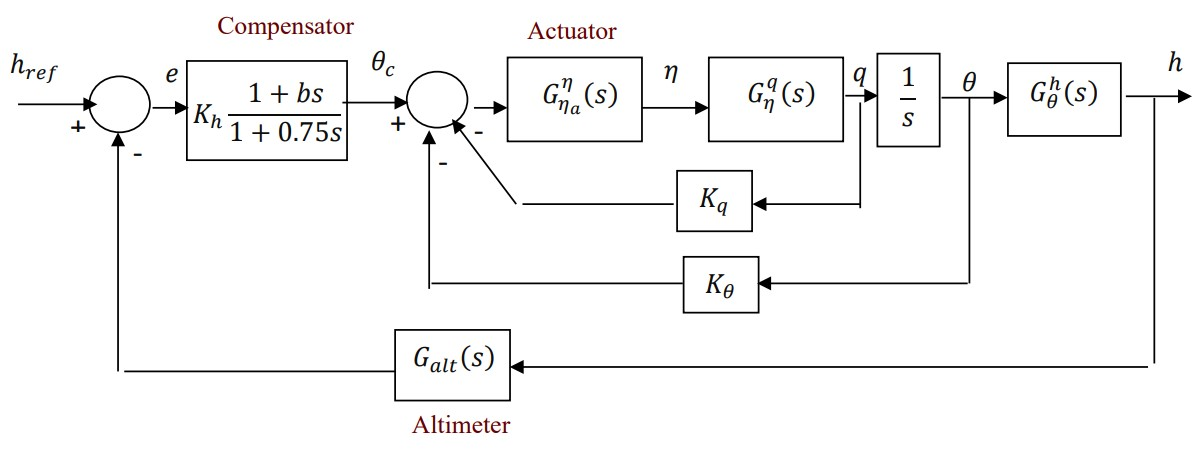
\includegraphics[width=1.1\textwidth]{pictures/figure 2.1.jpg}
\end{figure}

The first stage (inner loops) is responsible for regulating pitch attitude. It consists of both a pitch rate feedback loop, which damps excessive pitch rate variations, and a pitch angle feedback loop, which ensures the aircraft maintains required altitude by adjusting the elevator control. The closed loop transfer function for the pitch attitude design is derived by root locus design, to achieve a damping ratio of 0.5 and natural frequency of 3 rad/s. This is achieved as follows:

\begin{equation}
    s_{1} = -\sigma + j\omega_{d}
\end{equation}
\label{eq:2.8}
\myequations{Complex Number $s_1$}
\begin{equation}
    \sigma = \zeta\omega_{n}
\end{equation}
\label{eq:2.9}
\myequations{$\sigma$ In Terms of $\zeta$ and $\omega_n$}
\begin{equation}
    \omega_{d} = \omega_{n}\sqrt{1-\zeta^2}
\end{equation}
\label{eq:2.10}
\myequations{$\omega_d$ In Terms of $\zeta$ and $\omega_n$}

When $\zeta$ takes the value of 0.5 and $\omega_{n}$ takes the value of 3, $s_{1}=-1.5+2.5981j$.\newline

Then, a compensator zero is placed at $s=-a$ so that the desired pole lies on the root locus. This is achieved by first reducing the block diagram shown in figure 2, by replacing $G^\eta_{\eta_{a}}$ and $G^q_{\eta}$ with transfer function $G_{p}$.Finally transfer function $G_{1}$ can be found by dividing by $s$:

\begin{equation}
    G_{1} (s)={{G_{p}}\over{s_1}}
\end{equation}
\label{eq:2.11}
\myequations{Transfer Function $G_1$ - used to find compensator zero.}

Finally, the value of $a$ can be determined by ensuring that the sum of $a$ and the angle of $s_1$ multipled by the angle of $G_1$ is equal to $\pi$. This can be expressed mathematically as:

\begin{equation}
    \angle{((s_1+a)G_1 (s))}=\pi
\end{equation}
\label{eq:2.12}
\myequations{Expression for finding $a$}

With the compensator pole in place, values of the gains $K_q$ and $K_{theta}$ can be obtained, so that the closed-loop transfer function of the pitch attitude control system can be found.

\begin{equation}
    K_q={{1}\over{|G_1(s_1)|}}
\end{equation}
\label{eq:2.13}
\myequations{Equation for gain $K_q$}
\begin{equation}
    K_{\theta}=aK_q
\end{equation}
\label{eq:2.14}
\myequations{Equation for gain $K_{\theta}$}

So the closed-loop transfer function of the pitch attitude system is:

\begin{equation}
    G^{\theta}_{\theta_{c}}={{G_1 (s)}\over{1+K_q(s+a)G_1 (s)}}
\end{equation}
\label{eq:2.15}
\myequations{Transfer Function $G^{\theta}_{\theta_{ref}}$ - CLTF of pitch attitude system.}

The denominator of the transfer function in equation 2.15 is the characteristic equation of the pitch attitude system. This means that the zero of the system is located at  $s=-a$, with point $s_1$ lying on the root locus branch for the open loop transfer function: 

\begin{equation}
    G_2(s_1) = (s+a)G_1 (s)
    \label{eq:2.16}
\end{equation}
\myequations{Transfer Function $G_2$ - OLTF of pitch attitude system.}

This transfer function should also satisfy the root locus criterion, as the angular value should be exactly equal to $\pi$.

The second stage (outer loop) regulates the aircraft’s altitude by adjusting the pitch attitude. The altimeter provides altitude feedback, and a compensator adjusts the pitch command to correct altitude deviations. The altitude loop is only closed after designing the pitch control loop, so that appropriate pitch commands are generated, and then executed by the inner loop. Therefore, since the transfer function for the inner loop has been set (equation 2.15) the design for the outer loop can be determined by block diagram reduction, as seen in figure 2.2.

\begin{figure}[H]
    \caption{Simplified block diagram for the altitude hold loop (outer loop).}
    \label{fig:block_diagram_simplified_altitude_hold}
    \centering
    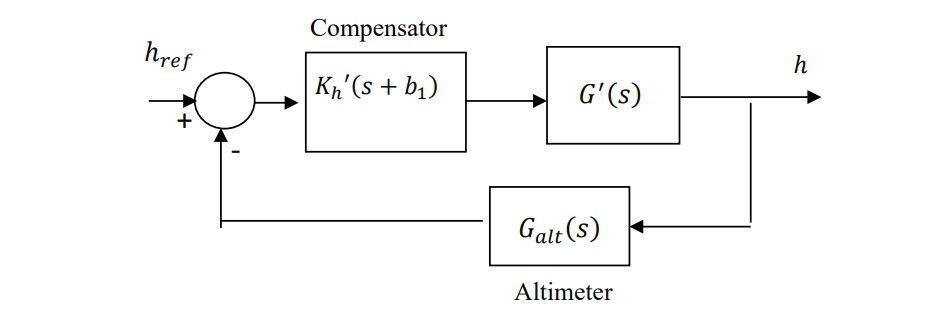
\includegraphics[width=1.1\textwidth]{pictures/figure 2.2.jpg}
\end{figure}

Where: 

\begin{equation}
    G^{\prime}= ({{1}\over{1+0.75s}})G^{\theta}_{\theta_{c}}(s)G^h_{\theta}(s)
    \label{eq:2.17}
\end{equation}
\myequations{Transfer Function $G^{\prime}$}

And: 

\begin{equation}
    G^*(s)=G^{\prime}(s)G_{alt}(s)
    \label{eq:2.18}
\end{equation}
\myequations{Transfer Function $G^{*}$}

Terms $K_h^{\prime}$ and $b_1$ are to be determined, however transfer function $G_{alt}(s)$ has known properties as the performance of the aircraft's elevators have been measured.

\begin{equation}
    G_{alt}(s)={{10}\over{s+10}}
    \label{eq:2.19}
\end{equation}
\myequations{Transfer Function $G_{alt}$}

For the outer loop, an identical method, to what was used in the inner loop, is used to design a root locus. The only difference is that we solve with complex number $s_2$ by using a $\zeta$ of 0.5 and a $\omega_n$ of 0.5 rad/s. Therefore, by recalling equations 2.8, 2.9 and 2.10, the complex number $s_2$ is found. Therefore, a compensator zero can be placed when $s=b_1$, which can be found by slightly modifying equation 2.12:

\begin{equation}
    \angle{((s_2+b_1)G^* (s_2))}=\pi
\end{equation}
\label{eq:2.20}
\myequations{Expression for finding $b_1$}

Once a suitable $b_1$ has been determined, the transfer function $G_3(s_2)$ can be determined, by taking $G_{alt}$ and multiplying by $(s+b_1)$, which now includes our compensator zero in the transfer function. This means that, the value of the gains $K_h^{\prime}$ and $K_h$ can be found by direct calculation:

\begin{equation}
    K_h^{\prime}={{1}\over{|G_3(s2)}}
\end{equation}
\label{eq:2.21}
\myequations{Expression for finding $K_h^{\prime}$}
\begin{equation}
    K_h={{K_h^{\prime}}\over{b_1}}
\end{equation}
\label{eq:2.22}
\myequations{Expression for finding $K_h$}

Additionally, just like for $G_2(s_1)$ the angular value of the transfer function $G_3(s2)$ should be exactly equal to $\pi$. 

Now, all unknown terms have been evaluated, including the gains used in the Compensator block in figure 2.2. This means that the outer loop can be closed around the inner loop, completing the theoretical altitude hold design. The simplified closed loop transfer function is:

\begin{equation}
    G_{h_c}^h(s)={{K_h^{\prime}(s+b_1)G^{\prime}}\over{1+G_3(s_2)K_h^{\prime}}}
\end{equation}
\label{eq:2.23}
\myequations{Closed loop transfer function of the altitude hold system.}

It's important to note the key relationship between the two loops: the inner loop must be fast and stable to respond effectively to pitch commands from the outer loop, whereas, the outer loop uses the inner loop to influence the altitude, but operates slower to avoid excessive oscillaitons. 

\subsection{Modelling and Results}
\subsection{Discussion}
\subsection{Conclusions}

\newpage
\section{Appendix}
\listoffigures
\listoftables
\listofmyequations

\newpage

\printbibliography

\end{document}